% vim: spell spelllang=da_dk

\documentclass[a4paper]{article}

\usepackage[a4paper,lmargin=0.8in,rmargin=0.8in,tmargin=1.1in]{geometry}

% Tekstindkodning og orddeling
\usepackage[utf8]{inputenc}
\usepackage[danish]{babel}

% Palatino skrifttype
\usepackage[T1]{fontenc}
\usepackage{mathpazo}
\renewcommand*{\arraystretch}{1.5}

\title{Koncerndiagram}
\author{Datalogisk Kantineforening}

% Fint hoved og fod
\usepackage{fancyhdr}
\usepackage{lastpage}
\renewcommand{\headrulewidth}{0in}
\setlength{\headheight}{20pt}
\pagestyle{fancy}
\makeatletter
\let\headtitle\@title
\let\headauthor\@author
\let\headdate\@date
\makeatother
\lhead{\headauthor}
\chead{\headtitle}
\rhead{\headdate}
\cfoot{Side \thepage{} af \pageref{LastPage}}
\fancypagestyle{first}{%
  \fancyhf{}%
  \cfoot{Side \thepage{} af \pageref{LastPage}}%
}

\usepackage{tikz}
\usetikzlibrary{positioning}

\usepackage{tabularx}

\newcommand{\underskrift}[0]{%
  \begin{tabular}{rlll}%
  Navn \\\cline{2-4}%
  Dato & \hspace{0.6in} & Sted & \hspace{0.9in} \\\cline{2-2}\cline{4-4}%
  Underskrift & \vspace{0.2in}\\\cline{2-4}%
  \end{tabular}%
}

\begin{document}

\maketitle
\thispagestyle{first}

\section*{\centering Bestyrelsen}

\newcommand{\formand}[0]{Niels Gustav Westphal Serup}
\newcommand{\fstkasserer}[0]{Mathias Grymer}
\newcommand{\sndkasserer}[0]{Oleksandr Shturmov}
\newcommand{\naestformand}[0]{Maria Bich Pham}

\begin{center}
\begin{tikzpicture}
\draw (0  , 0 ) node (formand) {\formand{} (formand)};
\draw (-3 , -1) node (fstkasserer) {\fstkasserer{} (kasserer)};
\draw (3  , -1) node (sndkasserer) {\sndkasserer{} (kasserer)};
\draw (0  , -2) node (tegning) %
  {$\uparrow$ (individuelt tegningsberettiget) $\uparrow$};
\draw[dashed] (-6, -2.5) -- (6, -2.5); 
\draw (0  , -3) node (tegning) %
  {$\downarrow$ (parvist tegningsberettiget) $\downarrow$};
\draw (0  , -4) node (naestformand) {\naestformand{} (næstformand)};
\draw[dashed] (-6, -4.5) -- (6, -4.5); 
\draw (0  , -5) node (menige) %
  {$\downarrow$ (menige bestyrelsesmedlemmer) $\downarrow$};
\draw (-3 , -6) node (truls) {Truls Asheim};
\draw (3  , -6) node (rene) {René Løwe Jacobsen};
\draw (-3 , -7) node (maja) {Maja Ling Han};
\draw (3  , -7) node (mikkel) {Mikkel Storgaard Knudsen};
\draw (-3 , -8) node (troels) {Troels Kamp Leskes};
\draw (3  , -8) node (vivien) {Vivien Lewkowicz de Neergaard};
\draw (-3 , -9) node (alexander) {Alexander Worm Olsen};
\draw (3  , -9) node (amalie) {Amalie Vangekjær};
\end{tikzpicture}
\end{center}

\section*{\centering Medlemskab}

\begin{center}

\begin{minipage}{0.7\textwidth}

\begin{center}

Som medlemmer kan optages enhver, som er ansat eller studerende \\ ved
Datalogisk Institut på Københavns Universitet. \\ Medlemskab tegnes for et
studieår af gangen.

\end{center}

\end{minipage}

\end{center}

\vspace{\fill}

\begin{center}

\begin{minipage}{0.5\textwidth}
\underskrift{}
\end{minipage}%
\begin{minipage}{0.5\textwidth}
\underskrift{}
\end{minipage}

\end{center}

\end{document}
